The training part contains six methods.

\begin{Code}
---------------------------------- python ----------------------------------
>>> romc.solve_problems(n1,
                        use_bo=False,
                        optimizer_args=None,
                        seed=None)
----------------------------------------------------------------------------                    
\end{Code}

\noindent
This method (a) draws the nuisance variables, (b) defines the
optimisation problems and (c) solves them using either a
gradient-based optimizer or Bayesian optimization. These tasks are
compleed sequentially, as shown in figure~\ref{fig:romc_overview}. The
definition of the optimisation problems is performed by drawing
\code{n_1} integer numbers from a discrete uniform distribution
$u_i \sim \mathcal{U}\{1, 2^{32}-1\}$. Each integer $u_i$ is the seed
used in \pkg{ELFI}'s random simulator. The seed $u_i$ is the
computational analogous of the random variables $\vb_i$, that were
defined in the previous chapter; freezing the \code{seed} absorbs all
the randomness of the simulator transforming it to a deterministic
function. Setting the argument \code{use_bo=True}, chooses the
Bayesian Optimisation scheme for obtaining $\thetab_i^*$. In this
case, apart from obtaining the optimal points $\thetab_i^*$, we also
fit a Gaussian Process (GP) as surrogate model $\hat{d}_i$. In this
scenario, in the following steps, $\hat{d}_i(\thetab)$ will replace
$g_i(\thetab)$ as the distance function.

\begin{Code}
---------------------------------- python ----------------------------------
>>> romc.distance_hist(**kwargs)
----------------------------------------------------------------------------  
\end{Code}

\noindent
This function helps the user decide which threshold $\epsilon$ to
use. It plots a histogram of the distances at the optimal point
$g_i(\thetab_i^*) : \{i = 1, 2, \ldots, n_1\}$ or $d_i^*$ in case
\code{use_bo=True}. The function accepts all keyword arguments and
forwards them to the underlying \code{matplotlib.hist()} function; in
this way the user may customise some properties of the histogram, such
as the number of bins or the range of values.

\begin{Code}
---------------------------------- python ----------------------------------  
>>> romc.estimate_regions(eps_filter,
                          use_surrogate=None,
                          region_args=None,
                          fit_models=False,
                          fit_models_args=None,
                          eps_region=None,
                          eps_cutoff=None)
----------------------------------------------------------------------------
\end{Code}

\noindent
This method constructs a bounding box around the optimal point
$\thetab_i^* : i = 1, 2, \ldots, n_1$ following
Algorithm~\ref{alg:region_construction}. The Hessian matrix is
approximated based on the Jacobian $\hess_i = \jac_i^T \jac_i$. The
eigenvectores are computed using the function
\code{numpy.linalg.eig()}. A check is performed so that the matrix
$\hess_i$ is not singular; if this is the case, the eigenvectors are
set to be the vectors of the standard Euclidean basis i.e.\
$\{ \mathbf{e_1} = (1, 0, \ldots), \mathbf{e_2} = (0,1,0,\ldots),
\text{etc} \}$. The limits of the bounding box are obtained by
repeteadly querying the distance function ($g_i(\thetab)$ or
$\hat{d}(\thetab)$) along the search directions given by $\hess_i$.

\begin{Code}
---------------------------------- python ----------------------------------
>>> romc.fit_posterior(args*)  # training in a single call
>>> romc.visualize_region(i)   # acceptance region
>>> romc.compute_eps(quantile) # estimates ε
----------------------------------------------------------------------------
\end{Code}

\noindent
The function \code{fit_posterior} is a syntactic sugar for applying
\code{solve_problems} and \\ \code{estimate_regions} into a single
step. The function \code{visualize_region} can be used for plotting
the bounding box around the optimal point, when the parameter space is
$1D$ or $2D$. The argument \code{i} is the index of the corresponding
optimization problem i.e.\ $i<n_1$. \code{compute_eps} returns the
appropriate distance value $d_{i=\kappa}^*$ where
$\kappa = \lfloor \frac{quantile}{n} \rfloor$ from the collection
$\{ d_i^* \} \forall i = \{1, \ldots, n\}$ where $n$ is the number of
accepted solutions. It can be used to automate the selection of the
threshold $\epsilon$, e.g.\ \code{eps=romc.compute_eps(quantile=0.9)}.


\subsubsection*{Example}


In the following snippet, we put together the routines described above
to perform the training part at our running example.

\begin{Code}
------------------------------ python snippet ------------------------------
  # Trainining (fitting) part
  n1 = 500 # number of optimisation problems
  seed = 21 # seed for solving the optimisation problems
  eps = .75 
  use_bo = False # set to True for switching to Bayesian optimisation

  # Training step-by-step
  romc.solve_problems(n1=n1, seed=seed, use_bo=use_bo)
  romc.theta_hist(bins=100) # plot hist to decide which eps to use

  eps = .75 # threshold for the bounding box based on histogram inspection
  romc.estimate_regions(eps=eps) # build the bounding boxes

  romc.visualize_region(i=1) # for inspecting visually the bounding box

  # Equivalent one-line command
  # romc.fit_posterior(n1=n1, eps=eps, use_bo=use_bo, seed=seed)
----------------------------------------------------------------------------  
\end{Code}

In figure \ref{fig:example_training_hist} we illustrate the
distribution of the distances obtained and the acceptance area of the
first optimisation problem. We observe that most optimal points
produce almost zero distance.

% \begin{figure}[h]
%   \begin{center}
%     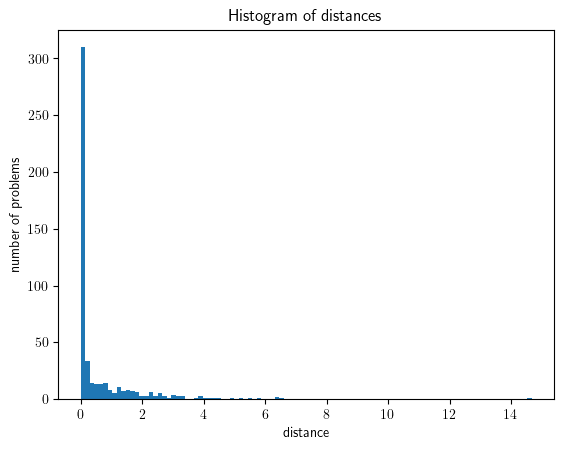
\includegraphics[width=0.48\textwidth]{./latex_files/images/chapter3/example_theta_dist.png}
%     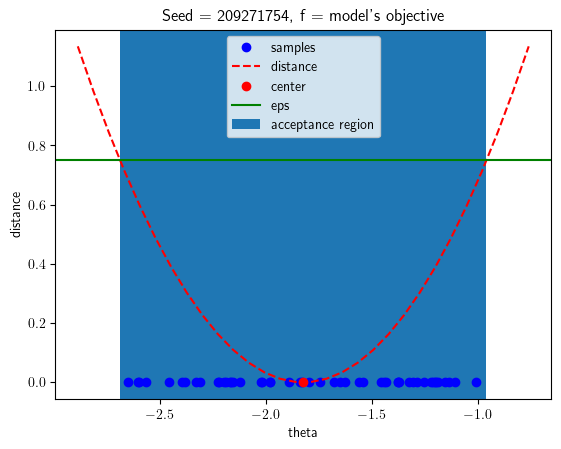
\includegraphics[width=0.48\textwidth]{./latex_files/images/chapter3/example_region_samples.png}
%     \end{center}
%     \caption[Histogram of distances at the 1D example.]{Histogram of
%       distances and visualisation of a specific region.}
%     \label{fig:example_training_hist}
% \end{figure}


\begin{figure}[h]
  \begin{center}
    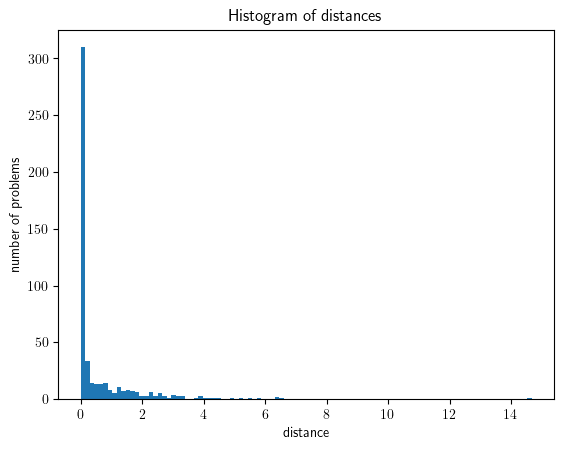
\includegraphics[width=0.32\textwidth]{./latex_files/images/chapter3/example_theta_dist.png}
    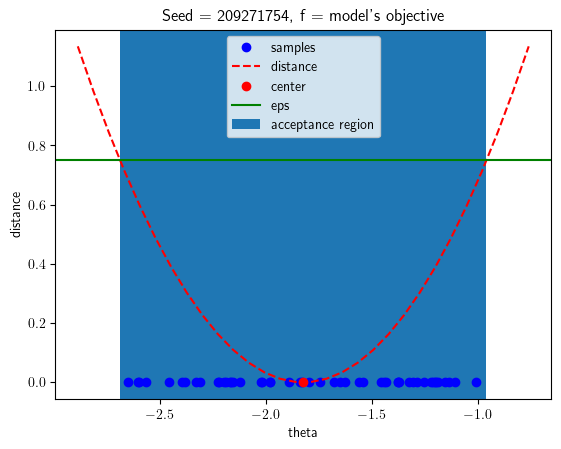
\includegraphics[width=0.32\textwidth]{./latex_files/images/chapter3/example_region_samples.png}
    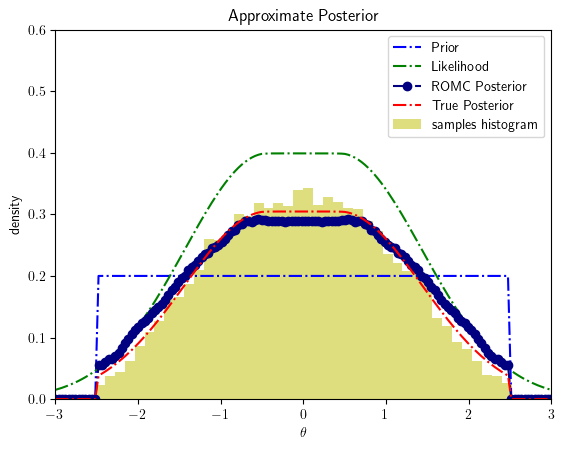
\includegraphics[width=0.32\textwidth]{./latex_files/images/chapter3/example_posterior.png}

    \end{center}
    \caption[Histogram of distances at the 1D example.]{Histogram of
      distances and visualisation of a specific region.}
    \label{fig:example_training_hist}
\end{figure}

